% ==============================================================================
% =================================== Aufgabe 5 =================================
% ==============================================================================

\chapter{Aufgabe}
\label{chap:5 Aufgabe}
\thispagestyle{fancy}
\section*{} 
\begin{figure}[h]
    \centering
    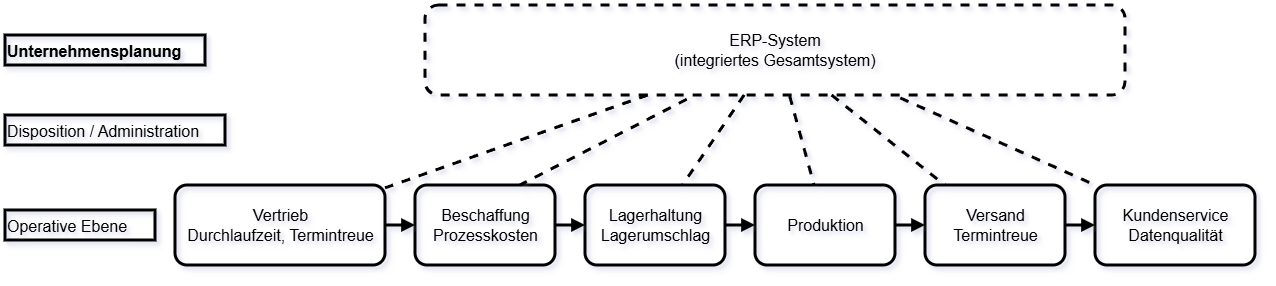
\includegraphics[width=0.95\textwidth]{./asset/image/ERP-Prozesse.png}
    \caption{Übersicht der \acs{ERP}-unterstützten Prozesse und Kennzahlen}
    \label{fig:erpprozess}
    [Quelle: Eigene Darstellung]
\end{figure}
In Anlehnung an die von Goram \cite[9]{29} dargelegte Charakterisierung des \acs{ERP}-Systems als integratives Rückgrat der betrieblichen Informationsverarbeitung wurden für die XYZ AG fünf Kennzahlen ausgewählt, um die Leistungsfähigkeit des Systems objektiv zu bewerten. Wie Gronau \cite[262]{13} im Kontext der strategischen Planung verdeutlicht, stützen sich diese Kennzahlen auf die horizontale und vertikale Integration des Unternehmens und ermöglichen so eine transparente Abbildung der prozessualen Auswirkungen. \par Die Einbettung der operativen Kernprozesse in die horizontale und vertikale Integrationsstruktur des ERP-Systems sowie die Zuordnung der zur Leistungsmessung gewählten Kennzahlen sind im Entwurf der \hyperref[fig:erpprozess]{Abbildung \ref{fig:erpprozess}} zusammenfassend dargestellt. \par \textbf{Übersicht der durch das \acs{ERP}-System unterstützten Prozesse}
\begin{itemize}
    \item \textbf{Materialwirtschaft und Logistik:} In seinem Grundlagenkapitel über die Bestandsführung und Logistik spezifiziert Gronau \cite[80]{8} zur Materialwirtschaft und Logistik die zentralen Komponenten, die von der \uline{Materialbedarfsplanung (\textit{\acs{MRP}})} über den (\textit{gesamten Einkaufszyklus} bis hin zur (\textit{Echtzeit-Lagerverwaltung}) und \uline{Rechnungsprüfung} reichen.
    \item \textbf{Produktion:} Das System unterstützt die \uline{Produktionsplanung} und \uline{-steuerung (\textit{\acs{PPS}})}, die Erstellung von \uline{Stücklisten} und \uline{Arbeitsplänen} sowie das Management von Fertigungskapazitäten sowohl in der Serien- als auch in der Einzelfertigung.
    \item \textbf{Vertrieb:} Wie Goram \cite[39]{30} im Rahmen der Geschäftsvorfälle im Vertrieb erläutert, werden hier Prozesse von der \uline{Akquisition}, über die \uline{Verfügbarkeitsprüfung (\textit{\acs{ATP}})} bis hin zur \uline{Auftragsabwicklung} und \uline{Fakturierung} abgebildet.
    \item \textbf{Rechnungswesen und Finanzen:} Hinsichtlich der Integration von Rechnungswesen und Finanzen betont Goram \cite[57]{31}, dass moderne \acs{ERP}-Systeme die \uline{Finanzbuchhaltung}, das \uline{Liquiditätsmanagement} sowie die \uline{Kosten-} und \uline{Leistungsrechnung} inklusive \uline{Controlling} nahtlos in den betrieblichen Wertefluss integrieren.
    \item \textbf{Personalwesen (\textit{\acs{HR}}):} Unterstützt werden die \uline{Personaladministration}, die \uline{Lohn-} und \uline{Gehaltsabrechnung}, die \uline{Zeitwirtschaft} (\textit{Zeiterfassung}) sowie die Personalbedarfsplanung und -entwicklung.
    \item \textbf{Querschnittsfunktionen:} Dazu zählen das \uline{Qualitätsmanagement} (\textit{Prüfplanung und -abwicklung}) sowie die \uline{Instandhaltung} von Betriebsmitteln.
\end{itemize}
\textbf{Fünf Kennzahlen zur Messung der Auswirkungen auf die Prozesse} \par Um die Effektivität und den Nutzen der \acs{ERP}-Einführung zu bewerten, können folgende Kennzahlen herangezogen werden:
\begin{enumerate}[label=\arabic*.), leftmargin=*]
    \item \textbf{Durchlaufzeit (\textit{\acs{z. B.} Bestellzyklus oder Auftragsabwicklungszeit}):} Durch die Automatisierung von Aktivitäten und die Eliminierung manueller Eingriffe können \acs{ERP}-Systeme (\textit{insbesondere im E-Procurement}) die \uline{Bestellzyklen um bis zu 70 \% verkürzen}.
    \item \textbf{Prozesskosten (\textit{Administrative Kosten}):} Hinsichtlich der auf die \uline{Reduzierung der administrativen Kosten} betont Goram \cite[19]{16}, dass die Standardisierung fragmentierter Abläufe den manuellen Datenpflegeaufwand erheblich reduziert, was Einsparungen (\textit{oft zwischen 41\% und 70\%}) ermöglichen kann.
    \item \textbf{Lagerumschlagshäufigkeit / Bestandskosten:} Eine verbesserte Disposition und Transparenz führt zu \uline{niedrigeren Lagerbeständen} und einer geringeren Kapitalbindung. Die Bestandskosten können durch optimierte Prognosemodelle signifikant gesenkt werden.
    \item \textbf{Termintreue (\textit{Liefertreue}):} Zur Messung der Termintreue (Liefertreue) werden die von Goram \cite[35]{32} beschriebenen Kriterien die \uline{Qualität logistischer Prozesse} herangezogen. Hierbei verbessert das \acs{ERP}-System die Logistik durch eine präzise Terminierung und rechtzeitige Prüfloseröffnung, was die Verlässlichkeit gegenüber dem Kunden maßgeblich steigert.
    \item \textbf{Datenqualität (\textit{Fehlerquote bei der Erfassung}):} Die Auswirkungen des Systems lassen sich an der \uline{Vermeidung von Erfassungs-} und \uline{Übertragungsfehlern} messen, da Daten nur einmal zentral erfasst werden und systemübergreifend konsistent zur Verfügung stehen.
\end{enumerate}

% ==============================================================================
% =================================== Aufgabe 5 =================================
% ==============================================================================